\documentclass{article}

%\usepackage{corl_2023} % Use this for the initial submission.
%\usepackage[final]{corl_2023} % Uncomment for the camera-ready ``final'' version.
\usepackage{corl_2023} % Uncomment for pre-prints (e.g., arxiv); This is like ``final'', but will remove the CORL footnote.

% ### custom packages start ###
% math
\usepackage{amsmath,amsfonts,amssymb,amsthm}
\usepackage{mathtools}
\usepackage{commath}
\DeclareMathOperator*{\argmax}{arg\,max}
\DeclareMathOperator*{\argmin}{arg\,min}

% tables
\usepackage{array}
\usepackage{booktabs}
\usepackage{multirow}

% figures
\usepackage{subcaption}
\usepackage{wrapfig}

% algorithms
\usepackage{algorithm}
\usepackage{algpseudocode}
\newcommand{\minuseq}{\mathrel{-}=}

% colors
\usepackage{color}  % CoRL uses color insted of xcolor.
\definecolor{purple}{rgb}{0.5,0.0,0.5}
\definecolor{olive}{rgb}{0.5,0.5,0.0}
% \newcommand{\ob}[1]{\textcolor{purple}{[\textbf{OB:} #1]}}
% \newcommand{\evdp}[1]{\textcolor{blue}{[\textbf{EvdP:} #1]}}
% \newcommand{\lsw}[1]{\textcolor{olive}{[\textbf{lsw:} #1]}}
% \newcommand{\rob}[1]{\textcolor{green}{[\textbf{rob:} #1]}}
% \newcommand{\tk}[1]{\textcolor{magenta}{[\textbf{TK:} #1]}}
% \newcommand{\rst}
% [1]{\textcolor{red}
% {[\textbf{ST:} #1]}}

% highlight
\usepackage{soul}
\definecolor{lightlightgrey}{rgb}{0.9,0.9,0.9}
\sethlcolor{lightlightgrey}

% notation
\newcommand{\pcx}[1]{\mathrm{X}^{(#1)}}
\newcommand{\wxy}[2]{W_{#1 \rightarrow #2}}
\newcommand{\bwxy}[2]{\bar{W}_{#1 \rightarrow #2}}
\newcommand{\vxy}[2]{V_{#1 \rightarrow #2}}
\newcommand{\pci}{\pcx{i}}
\newcommand{\pcj}{\pcx{j}}
\newcommand{\pcc}{\pcx{C}}
\newcommand{\wij}{\wxy{i}{j}}
\newcommand{\wci}{\wxy{C}{i}}
\newcommand{\bwci}{\bwxy{C}{i}}
\newcommand{\vci}{\vxy{C}{i}}

% ### custom packages end ###

% \title{SA-Warp: Simple $\mathrm{SE}(3)$ Object Re-arrangement \\via Shape and Action Warping}

% \title{Simple $\mathrm{SE}(3)$ Object Re-arrangement \\via Shape and Action Warping}

% didn't like the title above, but not sure how I feel about this one either...

% \title{One-Shot Imitation Learning via Shape Warping}

% \title{Imitation Learning via Simple Linear Shape Warping}
% \title{A Simple Method for Imitation Learning via Shape Warping}
\title{One-shot Imitation Learning via Interaction Warping}

% \title{Keypoint Matching via Linear Shape Warping}

% The \author macro works with any number of authors. There are two
% commands used to separate the names and addresses of multiple
% authors: \And and \AND.
%
% Using \And between authors leaves it to LaTeX to determine where to
% break the lines. Using \AND forces a line break at that point. So,
% if LaTeX puts 3 of 4 authors names on the first line, and the last
% on the second line, try using \AND instead of \And before the third
% author name.

% NOTE: authors will be visible only in the camera-ready and preprint versions (i.e., when using the option 'final' or 'preprint'). 
% 	For the initial submission the authors will be anonymized.

\author{
  Ondrej Biza$^1$, Skye Thompson$^2$, Kishore Reddy Pagidi$^1$, Abhinav Kumar$^1$, \\
  \textbf{Elise van der Pol$^{3,*}$, Robin Walters$^{1,*}$, Thomas Kipf$^{4,*}$} \\
  \textbf{Jan-Willem van de Meent$^{1,5,\dag}$, Lawson L.S. Wong$^{1,\dag}$, Robert Platt$^{1,\dag}$} \\
  $^1$ Northeastern University, $^2$ Brown University, $^3$ Microsoft Research, \\$^4$ Google DeepMind, $^5$ University of Amsterdam \\
  $^*$ Equal contribution. $^\dag$ Equal advising. \\
  \texttt{biza.o@northeastern.edu} \\
}

\begin{document}
\maketitle

%===============================================================================

\begin{abstract}
Imitation learning of robot policies from few demonstrations is crucial in open-ended applications. We propose a new method, Interaction Warping, for learning SE(3) robotic manipulation policies from a single demonstration. We infer the 3D mesh of each object in the environment using shape warping, a technique for aligning point clouds across object instances. Then, we represent manipulation actions as keypoints on objects, which can be warped with the shape of the object. We show successful one-shot imitation learning on three simulated and real-world object re-arrangement tasks. We also demonstrate the ability of our method to predict object meshes and robot grasps in the wild.
\end{abstract}

% Two or three meaningful keywords should be added here
\keywords{3D manipulation, imitation learning, shape warping.} 

%===============================================================================

\section{Introduction}

\begin{wrapfigure}[15]{r}{0.45\textwidth}
\vspace{-0.5cm}
  \begin{center}
    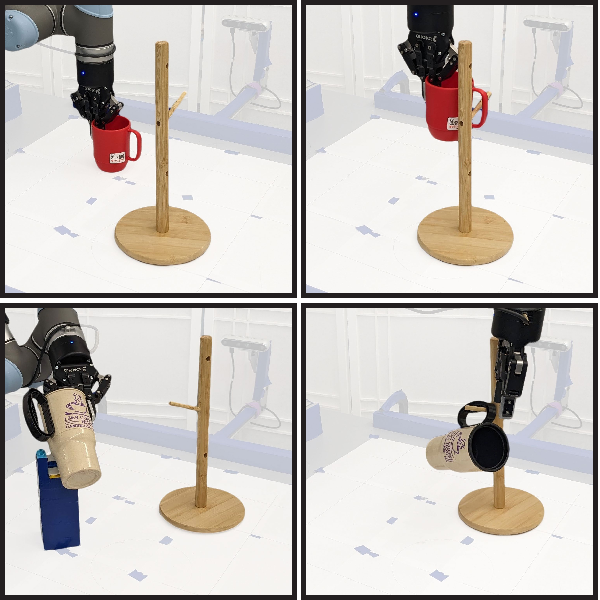
\includegraphics[width=0.4\textwidth]{figures/intro_2.pdf} \\
    \end{center}
\vspace{-0.2cm}
\caption{The Mug Tree task.}
\label{fig:mugontree}
\end{wrapfigure}


In one-shot imitation learning, we are given a single demonstration of a desired manipulation behavior and we must find a policy that can reproduce the behavior in different situations. A classic example is the Mug Tree task, where a robot must grasp a mug and hang it on a tree by its handle. Given a single demonstration of grasping a mug and hanging it on a tree (top row of Figure~\ref{fig:mugontree}), we want to obtain a policy that can successfully generalize across objects and poses, e.g. differently-shaped mugs and trees (bottom row of Figure~\ref{fig:mugontree}). This presents two key challenges: First, the demonstration must generalize to novel object instances, e.g. different mugs. Second, the policy must reason in $\mathrm{SE}(3)$, rather than in $\mathrm{SE}(2)$ where the problem is much easier \cite{wang22so2}. 

To be successful in $\mathrm{SE}(3)$ manipulation, it is generally necessary to bias the model significantly toward the object manipulation domains in question. One popular approach is to establish a correspondence between points on the surface of the objects in the demonstration(s) with the same points on the objects seen at test time. This approach is generally implemented using \emph{keypoints}, point descriptors that encode the semantic location of the point on the surface of an object and transfer well between different novel object instances~\cite{pan22taxpose,wang19dynamic,manuelli19kpam}. E.g., points on handles from different mugs should be assigned similar descriptors, thereby helping to correspond handles on different mug instances. A key challenge therefore becomes how to learn semantically meaningful keypoint descriptors. Early work used hand-coded feature labels~\cite{manuelli19kpam}.
%More recent methods learn descriptors during a pre-training step where category-level object descriptor models are trained using multiple in-category object instances over many categories.
More recent methods learn a category-level object descriptor models during a pre-training step
%This can be accomplished using implicit object models~\cite{simeonov2022neural} or point models~\cite{pan2022tax}. 
using implicit object models~\cite{simeonov22neural} or point models~\cite{pan22taxpose}. 

% More recent methods learn descriptors as the byproduct of an implicit object model~\cite{simeonov2022neural}. Other methods learn a point embedding using a constrastive loss on a DGCNN~\cite{wang2019dynamic} model~\cite{pan2022tax}. 

% This generally happens during a pretraining step where category-level object descriptor models are trained using a large number (generally hundreds) of in-category object instances for each category, e.g. hundreds of different instances of mugs. 

% The common thread here is that all of these methods involve a heavyweight category level object model that is trained on hundreds of objects to produce keypoint descriptors.

% keypoints~\cite{pan2022tax,wang2019dynamic,manuelli2019kpam}. The idea here is to train a neural network model to assign descriptors to points on a novel object instance as a function of their semantic location on the object, e.g. points on the handles from different mugs would be assigned similar descriptors. Once these descriptors have been learned, they can be used to represent relative object poses for object categories in terms of the relative locations of their keypoints. This enables us to translate a demonstration on one of set of in-category objects to a different set of in-category objects. For example, the system would be able to translate the demonstration in the top row of Figure~\ref{fig:mugontree} to produce the behavior in the bottom row of Figure~\ref{fig:mugontree}.

This paper proposes a different approach to the point correspondence problem based on Coherent Point Drift (CPD)~\cite{myronenko10pointset},
%a point-set registration algorithm.
a point-cloud warping algorithm.
We call this method \emph{Interaction Warping}. Using CPD, we train a shape-completion model to register a novel in-category object instance to a canonical object model in which the task has been defined via one-shot demonstration. The canonical task can then be projected into scenes with novel in-category objects by registering the new objects to the canonical models. Our method has several advantages over the previous work mentioned above~\cite{pan22taxpose,wang19dynamic,manuelli19kpam}. First, it performs better in terms of its ability to successfully perform a novel instance of a demonstrated task, both in simulation and on robotic hardware. Second, it requires an order-of-magnitude fewer object instances to train each new object category -- tens of object instances rather than hundreds.
%Third, our method is completely devoid of neural networks -- the approach is based on Gaussian Mixture models instead.
Third, our method is agnostic to the use of neural networks -- the approach presented is based on CPD and PCA models, though using neural networks is possible.% This makes the approach more computationally efficient \evdp{do you have an estimate of how much more?} and it means that it is much easier to reason about issues like uncertainty and safety of the model. 

%-- make sure we talk about novel instances, but known categories, i.e. category level manipulation

\section{Related Work}

% First paragraph about how our work is inspired by keypoints and how it relates to prior work on shape warping. Highlight the differences / novelty.
% Second paragraph on keypoints. Add a note about other imitation learning methods of 3D manipulation, such as PerAct. Add a note about zero-shot learning, PALM-E.
% Third paragraph on shape warping.
The two main lines of work we draw on are shape warping \cite{rodriguez18transferring,thompson21shapebased} and imitation learning via keypoints \cite{manuelli19kpam}. Shape warping uses non-rigid point cloud registration \cite{huang21comprehensive}, a set of methods for aligning point clouds or meshes of objects, to transfer robot skills across object of different shape. In this context, our paper is the first to use shape warping to perform relational object re-arrangement and to handle objects in arbitrary poses. Second, keypoints are a state abstraction method that reduces objects states to the poses of a set of task-specific keypoints.
%For example, relevant keypoints on a mug might be points on the rim and the handle of the mug. Keypoints are then used to transfer robotic policies to novel objects by matching their key points to the demonstration.
We use a version of keypoints, which we call interaction points, to transfer robot actions. The novelty in our work is that our interaction points are found automatically and warped together with object shape.

\textbf{Few-shot Learning of Manipulation Policies:} Keypoint based methods have been used in few-shot learning of object re-arrangement \cite{manuelli19kpam,gao21kpam,gao21kpamsc}. These methods rely on human-annotated object keypoints, which can be time-consuming to collect. Our work does not require manual annotation. Follow-up works proposed learned keypoints for learning tool affordances \cite{qin20keto,vecerik20s3k,turpin21gift} and for model-based reinforcement learning \cite{manuelli20keypoints}. A related idea is the learning of 2D \cite{florence18dense} and 3D \cite{simeonov22neural,simeonov22se,ryu22equivariant,chun23local} descriptor fields, which provide a semantic embedding for any point on an object. An arbitrary key point can then be matched across object instances using its embedding. We specifically compare to \citet{simeonov22neural,simeonov22se} and show that our method requires fewer demonstrations. In separate lines of works, \citet{pan22taxpose} (also included in our comparison) tackled object re-arrangement using cross-attention \cite{vaswani17attention} between point clouds and \citet{wen22you} used pose estimation to solve precise object insertion tasks. %
%\citet{shridhar22perceiveractor} leveraged language embeddings to learn multi-goal $\mathrm{SE}(3)$ manipulation policies.

\textbf{Shape Warping and Manipulation:} We use a learned model of in-class shape warping originally proposed by \citet{rodriguez18learning}. This model was previously used to transfer object grasps \cite{rodriguez18transferring,rodriguez18transferringa,klamt18supervised} and parameters for skills such as pouring liquids \cite{thompson21shapebased} (previously explored by \cite{brandi14generalizing}). Our method jointly infers the shape and pose of an object; prior work assumed object pose to be either given \cite{thompson21shapebased} or detected using a neural pose detector \cite{klamt18supervised}. Gradient descent on both the pose and the shape was previously used by \citet{rodriguez18transferring,rodriguez18transferringa}, but only to correct for minor deviations in pose. A second related line of work focuses on detecting the contacts between a gripper and an object, and then warping the contact points to fit a novel object \cite{li07datadriven,benamor12generalization,hillenbrand12transferring,jakel12learning,stouraitis15functional,rodriguez18learning,pavlichenko19autonomous,tian19transferring}. Finally, point-cloud warping has been used to manipulate deformable objects \cite{lee15learning,schulman16learning}.

\section{Background}
\label{sec:background}

\paragraph{Coherent Point Drift (CPD)}

\begin{wrapfigure}[9]{r}{0.45\textwidth}
    \centering
    \vspace{-2.5em}
    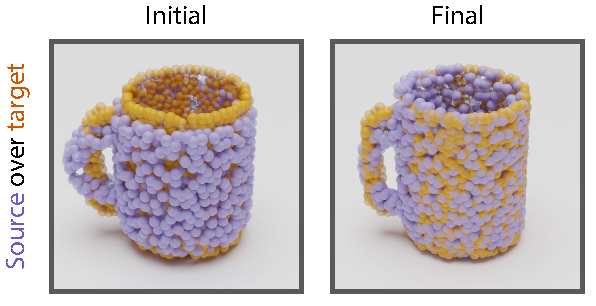
\includegraphics[width=0.45\textwidth]{figures/warping_small.pdf}
    \caption{Coherent Point Drift warping.}
    \label{fig:warping}
\end{wrapfigure}

Given two point clouds, $\pci \in \mathbb{R}^{n \times 3}$ and $\pcj \in \mathbb{R}^{m \times 3}$, Coherent Point Drift (CPD) finds a displacement $\wij  \in \mathbb{R}^{n \times 3}$ of the points $\pci$ that brings them as close as possible (in an $L_2$ sense) to the points $\pcj$~\cite{myronenko10pointset}. CPD is a non-rigid point-cloud registration method -- each point in $\pci$ can be translated independently. CPD minimizes the following cost function,
\begin{align} % OB: I'd like to remove this equation.
    J(\wij) = - \sum_{k=1}^{m} \log \sum_{l=1}^{n} \exp \left( \frac{1}{2 \sigma^2} \norm{\pci_l + (W_{i \rightarrow j})_l - \pcj_k } \right) + \frac{\alpha}{2} \phi(\wij),
\end{align}
using expectation maximization over point correspondences and distances (see~\cite{myronenko10pointset} for details). This can be viewed as fitting a Gaussian Mixture Model of $n$ components to the data $\pcj$. Here, $\phi(\wij)$ is a prior on the point displacements that regularizes nearby points in $\pci$ to move coherently, preventing the assignment of arbitrary correspondences between points in $\pci$ and $\pcj$.
% This incentivizes the optimization to not assign arbitrary correspondences between points in $\pci$ and $\pcj$.

\textbf{Generative Object Modeling Using CPD:} CPD can be used as part of a generative model for in-category object shapes as follows~\cite{rodriguez18transferring}. Assume that we are given a set of point clouds, $\{\pcx{1}, \dots, \pcx{K}\}$, that describe $K$ object instances that all belong to a single category, e.g. a set of point clouds describing different mug instances. Each of these point clouds must be a full point cloud in the sense that it covers the entire object. Select a ``canonical'' object $\pcx{C}, C \in \{1,2, ..., K\}$ and define a set of displacement matrices $\wxy{C}{i} = \mathrm{CPD}(\pcx{C}, \pcx{i}), i \in \{1, 2, ..., K\}$. The choice of $C$ is arbitrary, but we heuristically choose the $C$ that is the most representative (Appendix \ref{appendix:method:canonical}). Now, we calculate a low rank approximation of the space of object-shape deformations using PCA. For each matrix $\wxy{C}{i} \in \mathbb{R}^{n \times 3}$, let $\bwxy{C}{i} \in \mathbb{R}^{3n \times 1}$ denote the flattened version. We form the $3n \times K$ data matrix $\bar{W}_C = \left[\bwxy{C}{1}, \dots, \bwxy{C}{K}\right]$ and calculate the $d$-dimensional PCA projection matrix $W \in \mathbb{R}^{3n \times d}$. This allows us to approximate novel in-category objects using a low-dimensional latent vector $v_{\mathrm{novel}} \in \mathbb{R}^d$, which can be used to compute a point cloud
\begin{align}
Y = \pcc + \mathrm{Reshape}(W v_{\mathrm{novel}}),
\label{eq:background:warp}
\end{align}
where the $\mathrm{Reshape}$ operator casts back to an $n \times 3$ matrix.
%This is illustrated in Figure~\ref{fig:latent} where we show shapes generated by varying the first two principal components for the mug object category.

% Finally, we use PCA to solve for the matrix $W \in \mathbb{R}^{d \times n}$ that approximates $\wxy{C}{i} \approx \vxy{C}{i} W$ where $\vxy{C}{i} \in \mathbb{R}^{3 \times d}$ is a low dimensional representation ($d \ll n$) of $\wxy{C}{i}$. This allows us to approximate novel in-category objects as low dimensional matrix $\vxy{C}{novel}$: $\pcx{novel} = \pcc + \vxy{C}{novel} W$. This is illustrated in Figure~\ref{fig:latent} where we show shapes generated by varying the first two principle components for the mug object category.

\textbf{Shape Completion From Partial Point Clouds:} In practice, we want to be able to approximate complete point clouds for objects for which we only have a partial view~\cite{thompson21shapebased}. This can be accomplished using the generative model by solving for 
\begin{align}
    \mathcal{L}(Y) = \mathcal{D}(Y, \pcx{\mathrm{partial}}),
    \label{eq:background:loss}
\end{align}
using gradient descent on $v$. Essentially, we are solving for the latent vector that gives us a reconstruction closest to the observed points. To account for the partial view, \citet{thompson21shapebased} use the one-sided Chamfer distance \cite{barrow77parametric},
\begin{align}
    \mathcal{D}\left( \pci, \pcj \right) = \frac{1}{m} \sum_{k=1}^{m} \min_{l \in \{1, ..., n\}} \norm{ \pci_l - \pcj_k }_2.
    \label{eqn:chamfer}
\end{align}
Note that $\pci \in \mathbb{R}^{n \times 3}$ and $\pcj \in \mathbb{R}^{m \times 3}$ do not need to have the same number of points ($n \neq m$).
% In order to minimize Equation~\ref{eqn:chamfer} with respect to $\wij$, 

% Finally, the term $Wv$ can be replaced by a more expressive model, e.g. an auto-encoder \cite{thompson21shapebased} or possibly a diffusion model \cite{nichol22pointe}. We use PCA for simplicity.

% \subsection{asdf}

% Shape warping aims to find the correspondence between the shape of two objects by altering one shape to fit the other (Figure \ref{fig:warping}). Usually, the first step is to turn both objects into point clouds. This can be accomplished by sampling the surface or the volume of the object, or directly using the vertices that make up the mesh of the object. Given a pair of point clouds to be matched, shape warping draws on the literature of non-rigid point cloud registration \cite{huang21comprehensive}. Next, we outline the Coherent Point Drift algorithm \cite{manuelli20keypoints}, a common method for aligning a pair of point clouds. We also introduce the necessary notation we will use throughout the paper.

% Denote a pair of point clouds $\pci$ and $\pcj$. We want to compute a matrix of displacements $\wij$ that minimizes some distance function between $\pci + \wij$ and $\pcj$, such as the one-sided Chamfer distance:
% \begin{align}
%     d\left( \pci + \wij, \pcj \right) = \frac{1}{|\pcj|} \sum_{k=1}^{|\pcj|} \min_{l=1}^{|\pci|} \norm{ \pci_l + W_{i \rightarrow j, l} - \pcj_k }_2.
% \end{align}
% Note that the two point clouds can have a different number of points. In general, $\wij$ can re-arrange $\pci$ in an arbitrary way, leading to a mapping that is not useful. The Coherent Point Drift (CPD) algorithm regularizes $\wij$ so that nearby points in $\pci$ are displaced similarly. CPD formulates the problem as a fitting of a Gaussian Mixture Model (GMM), where $\pci$ is a set of components and $\pcj$ is the data. It uses expectation maximization to optimize the objective function
% \begin{align}
%     J(\wij) = - \sum_{k=1}^{|\pcj|} \log \sum_{l=1}^{|\pci|} \exp \left( \frac{1}{2 \sigma^2} \norm{\pcj_k - (\pci + \wij)_l} \right) + \frac{\alpha}{2} \phi(\wij).
% \end{align}
% The regularizer $\phi$ penalizes high frequencies in $\wij$, so that the displacements applied to $\pci$ do not oscillate among nearby points.

% \citet{rodriguez18transferring} observed that we can treat each displacement matrix $\wij$ as a data point in order to learn a generative model of object shapes. Given a canonical object $\pcc$ and a set of warps $\{ \wci \}_{i=1}^K$, each matrix $\wci$ is flattened and treated as a feature vector. Then, we fit a PCA projection matrix $W \in \mathbb{R}^{|\pcc|{\times}D}$ to the data, which allows us to represent each shape by a low-dimensional latent vector $v$:
% \begin{align}
%     \pcx{v} = \pcc + W v.
% \end{align}
% Given a new point cloud $\pci$, we infer its shape by solving the following optimization problem by gradient descent:
% \begin{align}
%     v^* = \argmin_{v \in \mathbb{R}^D} d(\pcc + W v, \pci).
% \end{align}
% Finally, the term $Wv$ can be replaced by a more expressive model, e.g. an auto-encoder \cite{thompson21shapebased} or possibly a diffusion model \cite{nichol22pointe}. We use PCA for simplicity.


\section{Interaction Warping}

\begin{figure}[b!]
    \centering
    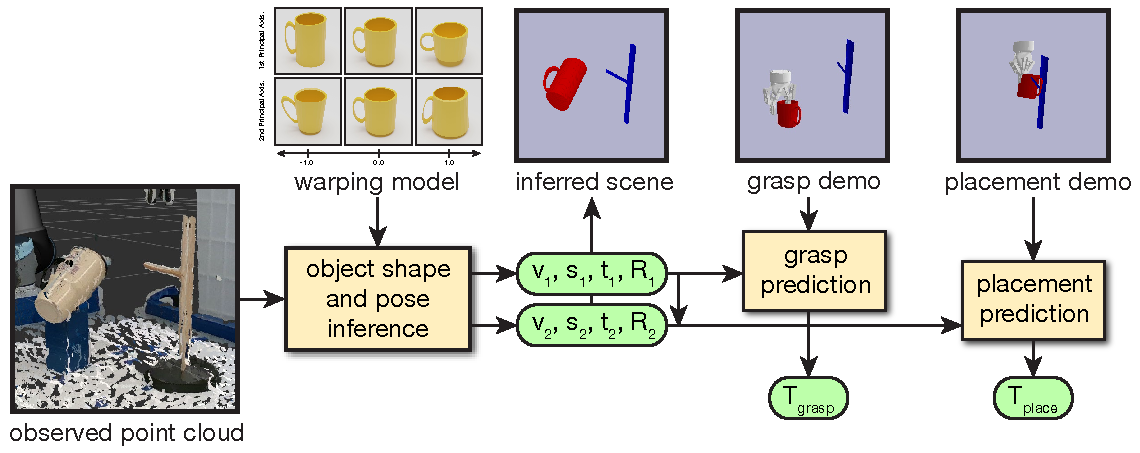
\includegraphics[width=0.9\textwidth]{figures/main_figure2.pdf}
    \caption{Interaction Warping pipeline for predicting grasp and placement poses from point clouds.}
    \label{fig:main}
\end{figure}

This section describes \textbf{Interaction Warping (IW)}, our proposed imitation method (Figure \ref{fig:main}). We assume that we have first trained a set of category-level generative object models of the form described in Section~\ref{sec:background}. Then, given a single demonstration of a desired manipulation activity, we detect the objects in the demonstration using off-the-shelf models. For each object in the demonstration that matches a previously trained generative model, we fit the model to the object in order to get the pose and completed shape of the object (Section \ref{sec:methods:scene} and \ref{sec:methods:mesh}).
%Next, for each grasp or placement, we project the relative poses of the objects involved onto the canonical models for the relevant object categories (Section \ref{sec:methods:cloning}).
Next, we identify \emph{interaction points} on pairs of objects that interact and corresponding those points with the matching points in the canonical object models. Finally, we reproduce the demonstration in a new scene with novel in-category object instances by projecting the demonstrated interaction points onto the completed object instances in the new scene (Section \ref{sec:methods:cloning}).

\subsection{Joint Shape and Pose Inference}
\label{sec:methods:scene}

In order to manipulate objects in $\mathrm{SE}(3)$, we want to jointly infer the pose and shape of an object represented by a point cloud $\pcx{\mathrm{partial}}$.
%We observe a real-world (or simulated) point cloud using one to three RGB-D cameras and we fuse the outputs into a single point cloud. We detect each object of interest in the point cloud either using clustering and heuristics (Section \ref{sec:exp:rearrangement}) or using pre-trained RGB-based open-vocabulary object detection and instance segmentation models (Section \ref{sec:exp:wild}).
% We infer the pose and shape of point cloud $Y \in \mathbb{R}^{n \times 3}$ by minimizing a loss function,
To do so, we warp and transform point cloud $Y \in \mathbb{R}^{n \times 3}$ to minimize a loss function,
\begin{align}
    \mathcal{L}(Y) = \mathcal{D}(Y, \pcx{\mathrm{partial}}) + \beta \max_k \norm{Y_k}_2^2,
\end{align}
which is akin to Equation \ref{eq:background:loss} with the addition of the second term, a regularizer on the size of the decoded object. Our implementation regularizes the object to fit into the smallest possible ball.
% Other options are possible, such as directly regularizing $v$ and $s$, regularizing the $L_2$ norm of $Y$, etc.
The main reason for the regularizer is to prevent large predicted meshes in real-world experiments, which might make it impossible to find collision-free motion plans.

We parameterize $Y$ as a warped, scaled, rotated and translated canonical point cloud,
\begin{align}
    Y = [\underbrace{(\pcc + \mathrm{Reshape}(W v))}_{\text{Equation } \ref{eq:background:warp}} \odot s] R^T + t.
    \label{eq:method:warp}
\end{align}
Here, $\pcc$ is a canonical point cloud and $v \in \mathbb{R}^d$ parameterizes a warped shape (as described in Section \ref{sec:background}), $s \in \mathbb{R}^3$ represents scale, $R \in \mathrm{SO}(3)$ is a rotation matrix and $t \in \mathbb{R}^3$ represents translation. We treat $s$ and $t$ as row vectors in this equation.

We directly optimize $\mathcal{L}$ with respect to $v, s$ and $t$ using the Adam optimizer \cite{kingma17adam}. We parameterize $R$ using $\hat{R} \in \mathbb{R}^{2 \times 3}$, an arbitrary matrix, and perform Gram-Schmidt orthogonalization (Algorithm \ref{alg:gram_schmidt}) to compute a valid rotation matrix $R$. This parameterization has been shown to enable stable learning of rotation matrices \cite{falorsi18explorations, park22learning}. We run the optimization with many initial random restarts, please see Appendix \ref{appendix:method:inference} for further details.

The inferred $v, s$ represent the shape of the object captured by $\pcx{\mathrm{partial}}$ and $R, t$ represent its pose.

\subsection{From Point Clouds to Meshes}
\label{sec:methods:mesh}

We infer the shape and pose of objects using point clouds, but we need object meshes to perform collision checking. This is important for finding contacts between objects and performing motion planning (Section \ref{sec:methods:cloning}). We propose a simple approach for recovering the mesh of the warped object based on the vertices and faces of the canonical object.

First, we need to warp the vertices of the canonical object. To do so, the vertices need to be a part of $\pcc$ because our model only knows how to warp points in $\pcc$ (Section \ref{sec:background}). However, these vertices (extracted from meshes made by people) are usually very biased (e.g. 90\% of the vertices might be in the handle of a mug), which results in learned warps that are ignore some parts of the object. Second, we add points to $\pcc$ that are randomly sampled on the surface of the canonical mesh. $\pcc$ is then composed of approximately the same number of mesh vertices and random surface samples, leading to a better learned warping. We construct $\pcc$ such that the first $V$ points are the vertices; note that the ordering of points in $\pcc$ does not change as it is warped.

Given a warped, rotated and translated point cloud $Y$ (Equation \ref{eq:method:warp}), the first $V$ points are the warped mesh vertices. We combine them with the faces of the canonical object to create a warped mesh $M$. Faces are represented as triples of vertices and these stay the same across object warps.

\subsection{Transferring Robot Actions via Interaction Points}
\label{sec:methods:cloning}

\begin{figure}
    \centering
    \begin{subfigure}[b]{0.22\textwidth}
        \centering
        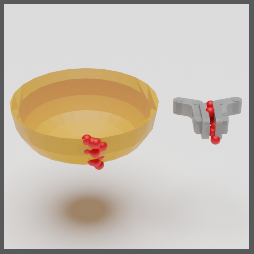
\includegraphics[width=\textwidth]{figures/contact_fig1.pdf}
        \caption{}
    \end{subfigure}
    \hspace{0.05\textwidth}
    \begin{subfigure}[b]{0.22\textwidth}
        \centering
        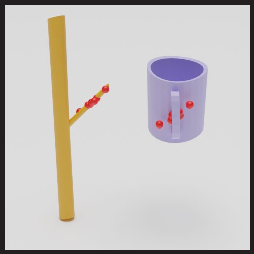
\includegraphics[width=\textwidth]{figures/contact_fig3.pdf}
        \caption{}
    \end{subfigure}
    \hspace{0.05\textwidth}
    \begin{subfigure}[b]{0.22\textwidth}
        \centering
        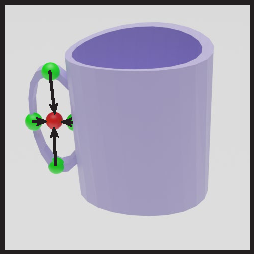
\includegraphics[width=\textwidth]{figures/contact_fig2.pdf}
        \caption{}
    \end{subfigure}
    \caption{(a) Contacts between a gripper and a bowl extracted from a demonstration. (b) Nearby points between a mug and a tree extracted from a demonstration of hanging the mug on the tree. (c) A virtual point (red) representing the branch of the tree intersecting the handle of the mug. The red point is anchored to the mug using k nearest neighbors on the mug (four are shown in green) and moves as the mug warps. All points shown in this visualization are extracted automatically.}
    \label{fig:contacts}
\end{figure}

\begin{figure}
    \centering
    \begin{subfigure}[b]{0.48\textwidth}
        \centering
        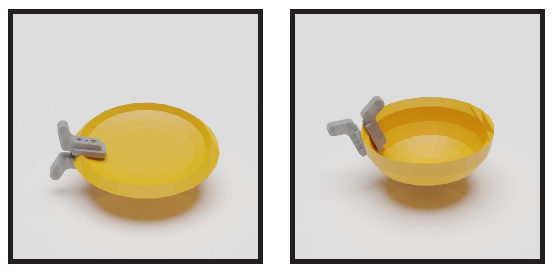
\includegraphics[width=\textwidth]{figures/picks_and_places_1.pdf}
        \caption{}
    \end{subfigure}
    \begin{subfigure}[b]{0.48\textwidth}
        \centering
        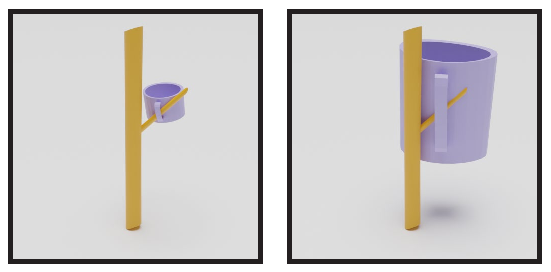
\includegraphics[width=\textwidth]{figures/picks_and_places_2.pdf}
        \caption{}
    \end{subfigure}
    % 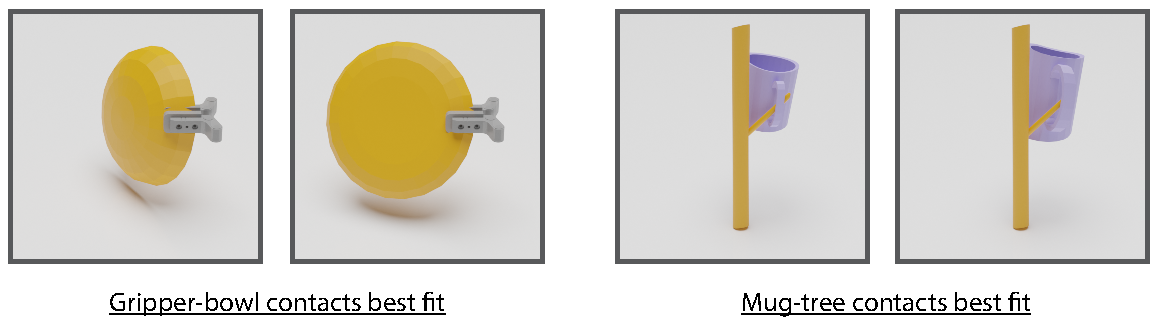
\includegraphics[width=\textwidth]{figures/picks_and_places.pdf}
    \caption{Predicting grasps using interaction point warping. (a) the predicted grasp for a bowl/plate changes based on the curvature of the object. (b) the placement of a mug on a mug tree changes as the mug grows larger so that the branch of the tree is in the middle of the handle.}
    \label{fig:grasps_and_placements}
\end{figure}

% \paragraph{Finding Interaction Points} Our key contribution is the idea of registering \textit{interaction points} onto a canonical mesh and transferring them to new object instances via shape warping. Consider a demonstration of a grasp with pose $T_{\mathrm{grasp}} \in \mathbb{R}^{4 \times 4}$. We infer the latent shape $v \in \mathbb{R}^{d}$ and pose $T$ of the grasped object as described in Section \ref{sec:methods:scene}. We also create a corresponding point cloud $\pcx{v}$ (Equation \ref{eq:dec}) and a mesh $\mathrm{obj}^{(v)}$.

% For grasping, we define interaction points as the contact points between the gripper and the object at the point of grasp. We use \texttt{pybullet} to find $N$ pairs of contact points $(p^{(v)}_i, p^{(G)}_i)$, where $p^{(v)}_i \in \pcx{v}$ and $p^{(G)}$ lies on the surface of the gripper mesh. Figure \ref{fig:contacts}(a) shows an example of interaction points for grasping a bowl. We further (un)transform the points $p^{(v)}$ so that they lie on the canonical mesh in a canonical pose,
% \begin{align}
%     p^{(C)}_i = \underbrace{T^{-1} p^{(v)}_i}_{(1)} - \underbrace{(\mathrm{Reshape}(Wv))_{i_j}}_{(2)},
% \end{align}
% where the first term transform the point into a canonical pose and the second term warps the point into the canonical shape. $i_j$ is the index of $p^{(v)}$ in $\pcx{v}$.

% For placement actions, we generalize the interaction points to include nearby points between a pair of objects. 

Consider the example of a point cloud of a mug $Y$ that is warped using Equation \ref{eq:method:warp}. We can select any point $Y_i$ and track it as the mug changes its shape and pose. For example, if the point lies on the handle of the mug, we can use it to align handles of mugs of different shapes and sizes. That can, in turn, facilitate the transfer of manipulation policies across mugs. The key question is how to find the points $Y_i$ relevant to a particular task. We call these \emph{interaction points}.

% We propose the idea of \textit{interaction points}, which are specific points on objects automatically found from a demonstration of a task. We use different techniques to find interaction points for object grasps and placements, and we describe them in turn.

\textbf{Grasp Interaction Points:} We define the grasp interaction points as the pairs of contact points between the gripper and the object at the point of grasp. Let $Y^{(A)}$ and $M^{(A)}$ be the point cloud and mesh respectively for the grasped object inferred by our method (Section \ref{sec:methods:scene}, \ref{sec:methods:mesh}). Let $M^{(G)}$ be a mesh of our gripper and $T_G$ the pose of the grasp. We use \texttt{pybullet} collision checking to find $P$ pairs of contact points $ (p_j^{(A)}, p_j^{(G)})_{j=1}^P$, where $p_j^{(A)}$ is on the surface of $M^{(A)}$ and $p_j^{(G)}$ is on the surface of $M^{(G)}$ in pose $T_G$ (Figure \ref{fig:contacts}a). We want to warp points $p_j^{(A)}$ onto a different shape, but our model only knows how to warp points in $Y^{(A)}$. Therefore, we find a set of indices $I_{G} = \{i_1,..., i_P\}$, where $Y^{(A)}_{i_j}$ is the nearest neighbor of $p^{(A)}_j$.

\textbf{Transferring Grasps:} In a new scene, we infer the point cloud of the new object $Y^{(A')}$ (Eq. \ref{eq:method:warp}). We solve for the new grasp as the optimal transformation $T_G^*$ that aligns the pairs of points $(Y^{(A')}_{i_j}, p^{(G)}_j), j \in \{1, ..., P\}, i_j \in I_G$. Here, $Y^{(A')}_{i_j}$ are the contact points from the demonstration warped to a new object instance. Note that there is a correspondence between the points in $Y^{(A)}$ and $Y^{(A')}$; shape warping does not change their order. We predict the grasp $T_G^*$ (Figure \ref{fig:grasps_and_placements}a) that minimizes the pairwise distances analytically using an algorithm from \citet{horn88computation}.

\textbf{Placement Interaction Points:} For placement actions, we look at two objects being placed in relation to each other, such as a mug being placed on a mug-tree. Here, we define interaction points as pairs of \textit{nearby points} between the two object, a generalization of contact points. We use nearby points so that the two objects do not have to make contact in the demonstration; e.g., the mug might not be touching the tree before it is released from the gripper. Similarly, the demonstration of an object being dropped into a container might not include contacts.

Let $Y^{(A)}$ and $Y^{(B)}$ be the inferred point clouds of the two objects. We capture the original point clouds from a demonstration right before the robot opens its gripper. We find pairs of nearby points with $L_2$ distance below $\delta$, $\{ (p^{(A)} \in Y^{(A)}, p^{(B)} \in Y^{(B)}) : \norm{p^{(A)} - p^{(B)}} < \delta \}$. Since there might be tens of thousands of these pairs, we find a representative sample using farthest point sampling \cite{eldar94farthest}. We record the indices of points $p^{(B)}_j$ in $Y^{(B)}$ as $I_P = \{ i_1, i_2, ..., i_P \}$.

We further add $p^{(B)}_j$ as \textbf{virtual points} into $Y^{(A)}$ -- this idea is illustrated in Figure \ref{fig:contacts} (b) and (c). For example, we wish to solve for a pose that places a mug on a tree, such that the branch of the tree intersects the mug's handle. But, there is no point in the middle of the mug's handle that we can use. Hence, we add the nearby points $p^{(B)}_j$ (e.g. points on the branch of the tree) as virtual points $q^{(A)}_j$ to $Y^{(A)}$. We anchor $q^{(A)}_j$ using L-nearest-neighbors so it warps together with $Y^{(A)}$. Specifically, for each point $p^{(B)}_j$ we find $L$ nearest neighbors $(n_{j,1}, ..., n_{j,L})$ in $Y^{(A)}$ and anchor $q^{(A)}_j$ as follows,
\begin{align}
    q^{(A)}_j = \frac{1}{L} \sum_{k=1}^L Y^{(A)}_{n_{j,k}} + \underbrace{(p^{(B)}_j - Y^{(A)}_{n_{j,k}})}_{\Delta_{j,k}} = p^{(B)}_j.
\end{align}
To transfer the placement, we save the neighbor indices $n_{j,k}$ and the neighbor displacements $\Delta_{j,k}$.

\textbf{Transferring Placements:} We infer the point clouds of the pair of new objects $Y^{(A')}$ and $Y^{(B')}$. We calculate the positions of the virtual points with respect to the warped nearest neighbors,
\begin{align}
    q^{(A')}_j = \frac{1}{L} \sum_{k=1}^L Y^{(A')}_{n_{j,k}} + \Delta_{j,k}.
\end{align}
We then construct pairs of points $(q^{(A')}_j, Y^{(B')}_{i_j}), j \in \{1, ..., P\}, i_j \in I_P$ and find the optimal transformation of the first object $T^*_P$ that minimizes the distance between the point pairs. Since we know how we picked up the first object, we can transform $T^*_P$ into the coordinate frame of the robot hand and execute the action of placing object $A'$ onto object $B'$ (Figure \ref{fig:grasps_and_placements}b).

% Our key contribution is a generalizable representation of 3D robotic actions with respect to manipulated objects. We propose an action abstraction we call \textit{interaction points}: pairs of these points capture the interaction of either a robot and an object, or a pair of objects. Crucially, we are able to warp interaction points to novel objects without any additional learning. We describe the cloning of grasping and relational object placement, but interaction points could be also used in, e.g., pushing or tossing. We use a single demonstration of a grasp or a placement to identify the interaction points.


% \paragraph{Warping Interaction Points}

% \paragraph{Using Multiple Demonstrations}

% \textbf{Grasping:} Assume that we have a single demonstration of grasping an object. We have inferred object shape $v$ and pose $T$ (Section \ref{sec:methods:scene}). We also have our reconstructed and transformed point cloud $\pcx{v}$, object mesh $\mathrm{obj}^{(v)}$ and a gripper mesh $\mathrm{grip}$. We find $N$ pairs of points $(p^{(v)}_j, p^{(G)}_j)$ that define the contacts between the object and the gripper. We use \texttt{pybullet} collision checking for this purpose. Each $p^{(v)}_j$ is a point in $\pcx{v}$ with index $i_j$.

% Given a new object to be grasped with shape $v'$, pose $T'$ and a point cloud $\pcx{v'}$, we create new pairs of points $(p^{(v')}_i, p^{(G)}_i)$. The points $p^{(v)}_i$ and $p^{(v')}_i$ \evdp{they're not in the below equation} are related by the following equation:
% \begin{align}
%     p^{(v')}_j T'^{-1} = \underbrace{p^{(v)}_j T^{-1}}_{\text{(1)}} + \underbrace{[W(v' - v)]_{i_j}}_{\text{(2)}} \label{eq:contact_point_warping}.
% \end{align}
% Intuitively, we transform the interaction points to a canonical pose and then warp them to conform to a new object instance. Term 1 ensures that we can repeat the grasp in any orientation ($\mathrm{SE}(3)$-invariance) and Term 2 encodes generalization over object shapes using linear shape warping.

% We compute the target pose of the robot gripper as the optimal transform $T_{\text{grasp}}$ of the points $p^{(G)}_j$ that minimizes the following loss function. An analytical solution exists \cite{horn88computation}.
% \begin{align}
%     \mathcal{L}(T) = \sum_{j=1}^N \norm{ p^{(v')}_j - T p^{(G)}_j }_2^2. \label{eq:coordinate_transform}
% \end{align}

% \textbf{Relational object placement:} We consider tasks where object 1 should be placed in a specific configuration relative to object 2. The placement can be both final (e.g. mug on mug-tree) or only a waypoint in a task (e.g. brush sliding over a canvas). Given a demonstration, we infer the pose $T_1, T_2$ and shape $v_1, v_2$ of both objects as well as their reconstructed and transformed point clouds $\pcx{v_1}, \pcx{v_2}$. We find all pairs of nearby points $(p^{(v_1)}_j \in \pcx{v_1}, p^{(v_2)}_j \in \pcx{v_2})$ such that $\norm{p^{(v_1)}_j - p^{(v_2)}_j} \leq \delta$. This step will usually return thousands of points and we find a subset of size 100 using farthest point sampling \cite{eldar94farthest} to get a representative sample. We use nearby points as a strict generalization of contact points: some demonstrations of a task can involve placing an object free of contact and letting it fall in place.

% Since $p^{(v_1)}_j$ and $p^{(v_2)}_j$ are not necessarily in contact, we cannot simply compute the optimal transform that aligns the pairs of points. We solve this problem by creating virtual points in $\pcx{v_1}$ that are in contact with points $p^{(v_2)}_j$. Each virtual point is defined as
% \begin{align}
%     p^{(v_1)}_{V,j} = \frac{1}{L} \sum_{k=1}^L \pcx{v_1}_{i_k} + \underbrace{(p^{(v_2)}_j - \pcx{v_1}_{i_k})}_{\Delta_k} = p^{(v_2)}_j,
% \end{align}
% where $i_1, i_2$, ..., $i_L$ are indices of the k-nearest-neighbors to point $p^{(v_2)}_j$ in $\pcx{v_1}$. Figure \ref{fig:contacts} (b) and (c) shows an example of this process: we create a virtual point in the middle of the handle of a mug, which is in contact with the branch of a mug-tree. Note that these points are found automatically and we do not require any task specific information.

% We now have pairs of points $(p^{(v_1)}_{V,j} \in \pcx{v_1}, p^{(v_2)}_j \in \pcx{v_2})$ that are in contact. Given a novel object 1 of shape $v'_1$, we can warp the virtual points as follows:
% \begin{align}
%     p^{(v'_1)}_{V,j} = \frac{1}{L} \sum_{k=1}^L \pcx{v'_1}_{i_k} + \Delta_k.
% \end{align}
% We can also warp the second object to shape $v'_2$ using Equation \ref{eq:contact_point_warping} and compute the new optimal transform $T_{\text{rel}}$ using Equation \ref{eq:coordinate_transform}. Finally, we transform $T_{\text{rel}}$ from the coordinate space of object 1 to the coordinate space of the gripper holding the object (we record the relative transform between the pose of the object and the gripper when we pick it up). Hence, we get $T_{\text{place}}$ that can be executed by a physical robot.

%Warping
% \subsection{Action: Warping of Grasps and Placements}
% \label{sec:methods:cloning}

% In this section, we describe our approach to clone pick and place actions for different object shapes and poses, given a single demonstration of a task. In general, the demonstration consists of a sequence of $T$ \evdp{is this symbol overloaded? Earlier in the paper capital T (with subscript) referred to transformations} pick and place actions manipulating $M$ objects. Our experiments are restricted to $T=M=2$, but our algorithm is immediately applicable to any sequence, as long as it is told which object to manipulate at which time step. We record the pose of the gripper and the inferred object shape and pose (using Algorithm \ref{alg:warp_infer}):
% \begin{align}
%     \left(T_{\text{pick/place}}, (v_k, T_k)_{k=1}^M\right)_{t=1}^T
% \end{align}

% \textbf{Grasp cloning:} To clone a grasp, we register contact points between the gripper and an object. Since we infer the mesh $X$ of the grasped object using Algorithm \ref{alg:warp_infer}, we can sample $B$ contact points between the object mesh and the gripper mesh (Figure \ref{fig:warping}a). For each contact point, we find the nearest neighbor in $X$. We record these indices as $\left< i_1, i_2, ..., i_B \right>$.

% When transferring the grasp to a new scene with a different object instance in a different position and orientation, we denote the completed point cloud of the new instance as $Y$. Points $Y_{i_1}, Y_{i_2}, ..., Y_{i_B}$ correspond to the points the gripper touched when picking up the demo object. Since the points have been warped to a new instance, a new grasp could be required. We solve for the best fit between the contact points on $Y$ and the contact points on the gripper (we have pairs of points, where the first point is on the object and the second on the gripper) to get a new grasp pose (Figure \ref{fig:grasps_and_placements}).

% \textbf{Placement cloning:} We consider the placement of a child object $X_{\mathrm{child}}$ on a parent object $X_{\mathrm{parent}}$ (e.g. mug on tree, bottle in box) \evdp{what is the definition of a child vs a parent object?}. Given the inferred meshes, we could find the contact points between the child and the parent. However, the two objects might not always touch before the child object is released from the gripper. E.g., when putting an object into a container. Instead, we find nearby points between the child and the parent and anchor them to the child point cloud as \textit{virtual points}.

% \rob{Exactly the same comment here as in the grasp section. 1) define the points we're looking for; 2) What properties do these points need to have such that placement is guaranteed to be successful? 3) Does our method deliver? When and when not?}

% We find points $p_1, p_2, ..., p_B$ on the parent object that are nearby the child object (Figure \ref{fig:contacts}b). These points are again found based on the inferred meshes of the two objects. For the parent object, we find a nearest neighbor $X_{\mathrm{parent},i_j}$ for each point $p_j$ -- it is the same process as in grasp cloning. For the child object, we anchor each point $p_j$ to its point cloud using its $K$ nearest neighbors $(n_1, n_2, ..., n_k)$. We save the deltas between $p_j$ and its neighbors $\delta = (v_j - n_1, v_j - n_2, ..., v_j - n_k)$ (Figure \ref{fig:contacts}c). Given warped nearest neighbors $n'$, we update $p_j$ as the mean over the deltas to the neighbors:
% \begin{align}
%     p'_j = \frac{1}{k} \sum_{i=1}^k n'_i + \delta_i.
% \end{align}

% Using the above method, we can calculate pairs of contact points in a novel scene. We solve for the transformation of the child object so that the contact points are in the best possible alignment with the target object. Finally, we solve for a collision free motion plan that places the child object to the target pose.

\section{Experiments}
\label{sec:exp}

We evaluate both the perception and imitation learning capabilities of Interaction Warping. In Section \ref{sec:exp:rearrangement}, we perform three object re-arrangement tasks with previously unseen objects both in simulation and on a physical robot. In Section \ref{sec:exp:wild}, we show our system is capable of proposing grasps in a cluttered kitchen setting from a single RGB-D image.

\subsection{Object Re-arrangement}
\label{sec:exp:rearrangement}

\begin{figure}[]
    \centering

    \begin{subfigure}{(\linewidth - 0.05\linewidth)/5}
        \centering
        \includegraphics[width=\linewidth]{figures/episodes/mug_on_tree_zoom/1.jpg}
    \end{subfigure}
    \begin{subfigure}{(\linewidth - 0.05\linewidth)/5}
        \centering
        \includegraphics[width=\linewidth]{figures/episodes/mug_on_tree_zoom/6.jpg}
    \end{subfigure}
    \begin{subfigure}{(\linewidth - 0.05\linewidth)/5}
        \centering
        \includegraphics[width=\linewidth]{figures/episodes/mug_on_tree_zoom/8.jpg}
    \end{subfigure}
    \begin{subfigure}{(\linewidth - 0.05\linewidth)/5}
        \centering
        \includegraphics[width=\linewidth]{figures/episodes/mug_on_tree_zoom/9.jpg}
    \end{subfigure}
    \begin{subfigure}{(\linewidth - 0.05\linewidth)/5}
        \centering
        \includegraphics[width=\linewidth]{figures/episodes/mug_on_tree_zoom/10.jpg}
    \end{subfigure}

    \caption{Example of an episode of putting a mug on a tree starting from a tilted mug pose.}
    \label{fig:mug_tree_episode_small}
\end{figure}

\begin{table*}[h]
    \centering
    \scalebox{0.92}{
    \begin{tabular}{lllcccccc}
        \toprule
          & \# & \# Train. & \multicolumn{2}{c}{\textbf{Mug on Tree}} & \multicolumn{2}{c}{\textbf{Bowl on Mug}} & \multicolumn{2}{c}{\textbf{Bottle in Container}} \\
         \textbf{Method} & Demo & Meshes & Upright & Arbitrary & Upright & Arbitrary & Upright & Arbitrary \\
         \midrule
         R-NDF \cite{simeonov22se} & 1 & 200 & 60.0 & 51.0 & 69.0 & 68.0 & 19.0 & 8.0 \\
         TAX-Pose \cite{pan22taxpose} & 1 & 200 & 61.0 & 41.0 & 16.0 & 9.0 & 4.0 & 1.0 \\
         \textbf{IW (Ours)} & 1 & 10 & \textbf{86.0} & \textbf{83.0} & \textbf{82.0} & \textbf{84.0} & \textbf{62.0} & \textbf{60.0} \\
         \midrule
         R-NDF \cite{simeonov22se} & 5 & 200 & 88.0 & \textbf{89.0} & 53.0 & 46.0 & 78.0 & 47.0 \\
         TAX-Pose \cite{pan22taxpose} & 5 & 200 & 82.0 & 51.0 & 29.0 & 14.0 & 6.0 & 2.0 \\
         \textbf{IW (Ours)} & 5 & 10 & \textbf{90.0} & 87.0 & \textbf{75.0} & \textbf{77.0} & \textbf{79.0} & \textbf{79.0} \\
         \midrule
         R-NDF \cite{simeonov22se} & 10 & 200 & 71.0 & 70.0 & 69.0 & 60.0 & \textbf{81.0} & 59.0 \\
         TAX-Pose \cite{pan22taxpose} & 10 & 200 & 82.0 & 52.0 & 20.0 & 20.0 & 2.0 & 1.0 \\
         \textbf{IW (Ours)} & 10 & 10 & \textbf{88.0} & \textbf{88.0} & \textbf{83.0} & \textbf{86.0} & 70.0 & \textbf{83.0} \\
         \bottomrule
    \end{tabular}
    }
    \caption{Success rates of predicted target poses of objects in \hl{simulation}. Upright and Arbitrary refer to the starting pose of the manipulated object. Measured over 100 trials with unseen object pairs.}
    \label{tab:simulation}
\end{table*}

\begin{table*}[t!]
    \centering
    \scalebox{0.92}{
    \begin{tabular}{lcccccc|cc}
         \toprule
          & \multicolumn{2}{c}{\textbf{Mug on Tree}} & \multicolumn{2}{c}{\textbf{Bowl on Mug}} & \multicolumn{2}{c}{\textbf{Bottle in Container}} & \multicolumn{2}{c}{\textbf{Mean}} \\
         \textbf{Method} & Pick & Pick\&Place & Pick & Pick\&Place & Pick & Pick\&Place & Pick & Pick\&Place \\
         \midrule
         NDF$^1$ \cite{simeonov22neural} & 93.3 & 26.7 & 75.0 & 33.3 & 20.0 & 6.7 & 62.8 & 22.2 \\
         R-NDF \cite{simeonov22se} & 64.0 & 12.0 & 37.5 & 37.5 & 26.7 & 20.0 & 42.7 & 23.2 \\
         \textbf{IW (Ours)} & \textbf{96.0} & \textbf{92.0} & \textbf{87.5} & \textbf{83.3} & \textbf{86.7} & \textbf{83.3} & \textbf{90.1} & \textbf{86.2} \\
         \bottomrule
    \end{tabular}
    }
    \caption{Success rates of \hl{real-world} pick-and-place experiments with a single demonstration. The manipulated object (e.g. a mug) starts in an arbitrary pose (we use a stand to get a range of poses) and the target object (e.g. a mug-tree) starts in an arbitrary upright pose. $^1$The target object (e.g. the mug tree) is in a fixed pose for this experiment, as NDF does not handle target object variation. Each entry is measured over 25 - 30 trials with unseen object pairs.}
    \label{tab:real_world}
\end{table*}

\textbf{Setup:} We use an open-source simulated environment with three tasks: mug on a mug-tree, bowl on a mug and a bottle in a  container \cite{simeonov22se}. Given a segmented point cloud of the initial scene, the goal is to predict the pose of the child object relative to the parent object (e.g.~the mug relative to the mug-tree). A successful action places the object on a rack / in a container so that it does not fall down, but also does not clip within the rack / container. The simulation does not test grasp prediction.

In our real-world experiment, we perform both grasps and placements based on a single demonstration. We capture a fused point cloud using three RGB-D. We use point-cloud clustering and heuristics to detect objects in the real-world scenes (details in Appendix \ref{appendix:experiment:rearrangement}) and perform motion planning with collision checking based on the meshes predicted by our method. We evaluate the ability of each method to pick and place unseen objects with a varying shape and pose (Figure \ref{fig:object_sets}).

\textbf{Result:} We find that our method (IW) generally outperforms R-NDF \cite{simeonov22neural} and TAX-Pose \cite{pan22taxpose} on the simulated relational-placement prediction tasks (Table \ref{tab:simulation}) with 20 times fewer training objects. We chose these two baselines as recent state-of-the-art $\mathrm{SE}$(3) few-shot learning methods.
% IW can succeed with one demonstration of a task, whereas R-NDF and TAX-Pose usually require five demonstrations.
IW can usually predict with above 80\% success rate even with 1 demo, whereas R-NDF and TAX-Pose can only occasionally do so with 5+ demos, and often fail to reach 80\% success rate at all.
We use an open-source implementation of R-NDF provided by the authors \cite{rndfgithub}, which differs in performance from the results reported in \cite{simeonov22se}. TAX-Pose struggles with precise object placements in the bowl on mug and bottle in box tasks; it often places the pair of objects inside one another.

In real-world pick and place experiments, we demonstrate the ability of IW to solve the three object re-arrangement tasks -- mug on tree, bowl on mug and bottle in box -- with unseen objects (Figure \ref{fig:object_sets}) and variation in the starting pose of objects (Table \ref{tab:real_world}). We find that NDF and R-NDF \cite{simeonov22neural,simeonov22se} struggle with the partial and noisy real-world point clouds. This often results in both the pick and place actions being too imprecise to successfully solve the task. Pre-training (R-)NDF on real-world point clouds could help, but note that IW was also pre-trained on simulated point clouds. We find that the warping of canonical objects is more robust to noisy and occluded point clouds. We show an example episode of placing a mug on a tree in Figure \ref{fig:mug_tree_episode_small}.

We use the meshes predicted by IW to perform collision checking during motion planning. We do not perform collision checking (other than to avoid contact with the table) when using (R-)NDF as these methods do not predict object meshes, but failures due to a collision between the robot and one of the object were infrequent in real-world (R-)NDF trials.

% \subsection{Trajectory Cloning}
% \label{sec:exp:trajectory}
% \textbf{Setup:} We record a single demonstration of a robot painting a particular pattern on a canvas with a brush. We then automatically segment this demonstration into waypoints and record the contact of the brush with the canvas at various waypoints. During testing, the robot uses a different brush and paints on a canvas that is potentially curved. We show that we can make predictions about the object poses that constitute the trajectory regardless of the shape of the brush and the canvas.
% \textbf{Result:} \ob{Abhinav}

\subsection{Grasp Prediction in the Wild}
\label{sec:exp:wild}

\begin{figure}[]
    \centering

    \begin{subfigure}{(\linewidth - 0.05\linewidth)/5}
        \centering
        \includegraphics[width=\linewidth]{figures/real2sim2real/2/1.png}
    \end{subfigure}
    \begin{subfigure}{(\linewidth - 0.05\linewidth)/5}
        \centering
        \includegraphics[width=\linewidth]{figures/real2sim2real/2/0.png}
    \end{subfigure}
    \begin{subfigure}{(\linewidth - 0.05\linewidth)/5}
        \centering
        \includegraphics[width=\linewidth]{figures/real2sim2real/2/3_sim.png}
    \end{subfigure}
    \begin{subfigure}{(\linewidth - 0.05\linewidth)/5}
        \centering
        \includegraphics[width=\linewidth]{figures/real2sim2real/2/3.png}
    \end{subfigure}
    \begin{subfigure}{(\linewidth - 0.05\linewidth)/5}
        \centering
        \includegraphics[width=\linewidth]{figures/real2sim2real/2/4.png}
    \end{subfigure}

    \begin{subfigure}{(\linewidth - 0.05\linewidth)/5}
        \centering
        \includegraphics[width=\linewidth]{figures/real2sim2real/5/1.png}
        \caption{}
    \end{subfigure}
    \begin{subfigure}{(\linewidth - 0.05\linewidth)/5}
        \centering
        \includegraphics[width=\linewidth]{figures/real2sim2real/5/0.png}
        \caption{}
    \end{subfigure}
    \begin{subfigure}{(\linewidth - 0.05\linewidth)/5}
        \centering
        \includegraphics[width=\linewidth]{figures/real2sim2real/5/3_sim.png}
        \caption{}
    \end{subfigure}
    \begin{subfigure}{(\linewidth - 0.05\linewidth)/5}
        \centering
        \includegraphics[width=\linewidth]{figures/real2sim2real/5/3.png}
        \caption{}
    \end{subfigure}
    \begin{subfigure}{(\linewidth - 0.05\linewidth)/5}
        \centering
        \includegraphics[width=\linewidth]{figures/real2sim2real/5/4.png}
        \caption{}
    \end{subfigure}

    \caption{Grasp prediction in the wild: (a) an RGB-D (depth not shown) image, (b) open-vocabulary object detection and segmentation using Detic \cite{zhou22detecting} and Segment Anything \cite{kirillov23segment}, (c) object meshes predicted by our method based on segmented point clouds (we filter out distant and small objects), (d) meshes projected into the original image, (e) grasps predicted by Interaction Warping projected into the original image. Figure \ref{fig:real2sim2real_part2} has additional examples.}
    \label{fig:real2sim2real}
\end{figure}

\textbf{Setup:} In this experiment, we show that we can combine our method with a state-of-the-art object detection and segmentation pipeline to predict object meshes and robot grasps from a single RGB-D image. We use an open-vocabulary object detector Detic \cite{zhou22detecting} to predict bounding boxes for common household objects and Segment Anything \cite{kirillov23segment} to predict segmentation masks within these bounding boxes. We turn the predicted RGB-D images into point clouds and use our shape warping model to predict a mesh for each object. Finally, we use interaction warping to predict a robot grasp based on a single demonstration per each object class (details in Appendix \ref{appendix:experiment:wild}).

\textbf{Result:} We show the results for two example scenes in Figure \ref{fig:real2sim2real} and \ref{fig:real2sim2real_part2}. Our perception pipeline can successfully detect objects in images with cluttered backgrounds. Our warping algorithm accounts for the variation in the shape and size of objects and our interaction warping algorithm can generalize the demonstrated grasps to the novel objects.

\section{Limitations and Conclusion}

We introduced Interaction Warping, a method for one-shot learning of $\mathrm{SE}$(3) robotic manipulation policies. We demonstrated that warping of shapes and interaction points leads to successful one-shot learning of object re-arrangement policies. We also showed that we can use open-vocabulary detection and segmentation models to detect objects in the wild and predict their meshes and grasps. 

\textbf{Limitations:} Our method requires segmented point clouds of objects. We demonstrated a pipeline for real-world detection in Section \ref{sec:exp:wild}, but it can be difficult to capture clean point clouds that align with RGB-based segmentation predictions. The process of jointly inferring shape and pose of an object takes around 25 seconds per object on a single desktop GPU. Future work could train an additional neural network to amortize the inference, or to predict favorable initialization. We use a PCA model of shape warps for simplicity; this model cannot capture the details of objects, such as the detailed shape of the head of a bottle. A model with higher capacity should be used for tasks that require high precision. Finally, our predicted policy is fully determined by the shape warping model and a single demonstration; our method does not learn from its failures, but it is fully differentiable.

%Future work could equip interaction warping with a more expressive shape warping model, so that it can predict 3D meshes of novel objects with high precision. Another interesting direction is to combine shape warping with object decomposition \cite{tenorth13decomposing,vahrenkamp16partbased,chen22neural} to learn representations of parts of complex objects, such as the door of a toaster oven or a water tank of a coffee machine. Shape warping could be used to represent articulated as well as deformable objects.

%===============================================================================

\clearpage

%===============================================================================

% no \bibliographystyle is required, since the corl style is automatically used.
\bibliography{main,zotero}  % .bib

\clearpage
\appendix

\section{Method Details}
\label{appendix:method}

We included the code for both our simulated and real-world experiments for reference. Please find it in the supplementary material under \texttt{iw\_code}. Algorithms \ref{alg:warp_learn} and \ref{alg:warp_infer} describe our warp learning and inference.

\begin{algorithm}[H]

\caption{Warp Learning}\label{alg:warp_learn} 

\begin{flushleft}
    \hspace*{\algorithmicindent} \textbf{Input:} Meshes of $K$ example object instances $\{ \mathrm{obj}_1, \mathrm{obj}_2, ..., \mathrm{obj}_K \}$. \\
    \hspace*{\algorithmicindent} \textbf{Output:} Canonical point cloud, vertices and faces and a latent space of warps. \\
    \hspace*{\algorithmicindent} \textbf{Parameters:} Smoothness of CPD warping $\alpha$ and number of PCA components $L$.
\end{flushleft}

\begin{algorithmic}[1]

    \State $\mathrm{PCD} = \left< \mathrm{SampleS}(\mathrm{obj}_i) \right>_{i=1}^K$. \Comment{\textcolor{blue}{Sample a small point cloud per object (Appendix \ref{appendix:method:sampling}).}}
    \State $C = \mathrm{SelectCanonical}(\mathrm{PCD})$. \Comment{\textcolor{blue}{Select a canonical object with index $C$ (Appendix \ref{appendix:method:canonical}).}}
    \State $\mathrm{canon} = \mathrm{Concat}(\mathrm{obj}_C.\mathrm{vertices}, \mathrm{SampleL}(\mathrm{obj}_C))$. \Comment{\textcolor{blue}{Use both vertices and surface samples.}}
    \For {$i \in \{ 1, 2, ..., K \}, i \neq C$}
        \State $W_{C \rightarrow i} = \mathrm{CPD}(\mathrm{canon}, \mathrm{PCD}_i, \alpha)$. \Comment{\textcolor{blue}{Coherent Point Drift warping (Section \ref{sec:background}).}}
    \EndFor
    \State $D_W = \{ \mathrm{Flatten}(W_{C \rightarrow i}) \}_{i = 1, i \neq C}^K$. \Comment{\textcolor{blue}{Dataset of displacements of $\mathrm{canon}$.}}
    \State $\mathrm{PCA} = \mathrm{FitPCA}(D_W, \mathrm{n\_components}=L)$. \Comment{\textcolor{blue}{Learn a latent space of canonical object warps.}}
    \State \Return $\mathrm{Canon}(\mathrm{points} = \mathrm{canon}, \mathrm{vertices} = \mathrm{obj}_C.\mathrm{vertices}, \mathrm{faces} = \mathrm{obj}_C.\mathrm{faces}), \mathrm{PCA}$.

\end{algorithmic}

\end{algorithm}

\begin{algorithm}[H]

\caption{Warp Inference and Mesh Reconstruction}\label{alg:warp_infer} 

\begin{flushleft}
    \hspace*{\algorithmicindent} \textbf{Input:} Observed point cloud $\mathrm{pcd}$, canonical object $\mathrm{canon}$ and latent space $\mathrm{PCA}$. \\
    \hspace*{\algorithmicindent} \textbf{Output:} Predicted latent shape $v$ and pose $T$. \\
    \hspace*{\algorithmicindent} \textbf{Parameters:} Number of random starts $S$, number of gradient descent steps $T$, learning rate $\eta$ and object size regularization $\beta$.
\end{flushleft}

\begin{algorithmic}[1]

    \State $t_g = \frac{1}{|\mathrm{pcd}|} \sum_{i=1}^{|\mathrm{pcd}|} \mathrm{pcd}_i$.
    \State $\mathrm{pcd} = \mathrm{pcd} - t_g$. \Comment{\textcolor{blue}{Center the point cloud.}}
    \For {$i = 1$ \textbf{to} $S$}
        \State $R_{\mathrm{init}} =$ Random initial 3D rotation matrix.
        \State Initialize $v = \begin{pmatrix} 0 & 0 & ... & 0 \end{pmatrix}, s = \begin{pmatrix} 1 & 1 & 1 \end{pmatrix}, t_l = \begin{pmatrix} 0 & 0 & 0 \end{pmatrix}, r = \begin{pmatrix} 1 & 0 & 0 \\ 0 & 1 & 0 \end{pmatrix}$.
        \State Initialize $\mathrm{Adam}$ \cite{kingma17adam} with parameters $v, s, t_l, r$ and learning rate $\eta$.
        \For {$j = 1$ \textbf{to} $T$}
            \State $\delta = \mathrm{Reshape}(Wv)$.
            \State $X = \mathrm{canon.points} + \delta$. \Comment{\textcolor{blue}{Warped canonical point cloud.}}
            \State $R = \mathrm{GramSchmidt(r)}$.
            \State $X = (X \odot s) R_{\mathrm{init}}^T R^T + t_l$. \Comment{\textcolor{blue}{Scaled, rotated and translated point cloud.}}
            \State $\mathcal{L} = \frac{1}{|\mathrm{pcd}|} \sum_k^{|\mathrm{pcd}|} \min_l^{|X|} \norm{\mathrm{pcd}_k - X_l}_2^2$. \Comment{\textcolor{blue}{One-sided Chamfer distance.}}
            \State $\mathcal{L} = \mathcal{L} + \beta \max_l^{|X|} \norm{X_l}_2^2$. \Comment{\textcolor{blue}{Object size regularization.}}
            \State Take a gradient descent step to minimize $\mathcal{L}$ using $\mathrm{Adam}$.
        \EndFor
    \EndFor
    \State Find parameters $v^*, s^*, t^*_l, R_{\mathrm{init}}^*, R^*$ with the lowest final loss across $i \in \{ 1, 2, ..., S \}$.
    \State $X = \mathrm{canon.points} +\mathrm{Reshape}(W v^*)$.
    \State $X = (X \odot s^*) (R_{\mathrm{init}}^*)^T (R^*)^T + t^*_l + t_g$. \Comment{\textcolor{blue}{Complete point cloud in workspace coordinates.}}
    \State $\mathrm{vertices} = \langle X_1, X_2, ..., X_{|\mathrm{canon.vertices}|} \rangle$. \Comment{\textcolor{blue}{First $|\mathrm{canon.vertices}|$ points of $X$ are vertices.}}
    \State \Return $\mathrm{Mesh}(\mathrm{vertices} = \mathrm{vertices}, \mathrm{faces} = \mathrm{canon.faces})$. \Comment{\textcolor{blue}{Warped mesh.}}

\end{algorithmic}

\end{algorithm} %\evdp{There is a lot of information here, is it possible to present the main steps here and leave the details for the appendix?}

\subsection{Point Cloud Sampling}
\label{appendix:method:sampling}

We use \texttt{trimesh}\footnote{https://github.com/mikedh/trimesh} to sample the surface of object meshes. The function \texttt{trimesh.sample.sample\_surface\_even} samples a specified number of points and then rejects points that are too close together. We sample 2k points for small point clouds ($\mathrm{SampleS}$) and 10k point for large point clouds ($\mathrm{SampleL}$).

\subsection{Canonical Object Selection}
\label{appendix:method:canonical}

Among the $K$ example objects, we would like to find the one that is the easiest to warp to the other objects. For example, if we have ten examples of mugs, but only one mug has a square handle, we should not choose it as it might be difficult to warp it to conform to the round handles of the other nine mugs. We use Algorithm \ref{alg:canon_select_1}, which computes $K * K-1$ warps and picks the object that warps to the other $K-1$ objects with the lowest Chamfer distance. We also note an alternative and computationally cheaper algorithm from \citet{thompson21shapebased}, Algorithm \ref{alg:canon_select_2}. This algorithm simply finds the object that is the most similar to the other $K-1$ objects without any warping.

\begin{algorithm}[H]

\caption{Exhaustive Canonical Object Selection}\label{alg:canon_select_1} 

\begin{flushleft}
    \hspace*{\algorithmicindent} \textbf{Input:} Point clouds of $K$ training objects $\langle \pcx{1}, \pcx{2}, ..., \pcx{K} \rangle$. \\
    \hspace*{\algorithmicindent} \textbf{Output:} Index of the canonical object. \\
\end{flushleft}

\begin{algorithmic}[1]

    \For {$i = 1$ \textbf{to} $K$}
        \For {$j = 1$ \textbf{to} $K$, $j \neq i$}
            \State $\wij = \mathrm{CPD}(\pci, \pcj)$ \Comment{\textcolor{blue}{Warp point cloud $i$ to point cloud $j$.}}
            \State $C_{i,j} = \frac{1}{|\pcj|} \sum_{k=1}^{|\pcj|} \min_{l=1}^{|\pci|} \norm{\pcj_k - (\pci + \wij)_l}_2^2$
        \EndFor
    \EndFor
    \For {$i = 1$ \textbf{to} $K$}
        \State $C_i = \sum_{j = 1, j \neq i}^K C_{i,j}$ \Comment{\textcolor{blue}{Cumulative cost of point cloud $i$ warps.}}
    \EndFor
    \State \Return $\argmin_{i=1}^K C_i$ \Comment{\textcolor{blue}{Pick point cloud that is the easiest to warp.}}

\end{algorithmic}

\end{algorithm}

\begin{algorithm}[H]

\caption{Approximate Canonical Object Selection \cite{thompson21shapebased}}\label{alg:canon_select_2} 

\begin{flushleft}
    \hspace*{\algorithmicindent} \textbf{Input:} Point clouds of $K$ training objects $\langle \pcx{1}, \pcx{2}, ..., \pcx{K} \rangle$. \\
    \hspace*{\algorithmicindent} \textbf{Output:} Index of the canonical object. \\
\end{flushleft}

\begin{algorithmic}[1]

    \For {$i = 1$ \textbf{to} $K$}
        \For {$j = 1$ \textbf{to} $K$, $j \neq i$}
            \State $C_{i,j} = \frac{1}{|\pcj|} \sum_{k=1}^{|\pcj|} \min_{l=1}^{|\pci|} \norm{\pcj_k - \pci_l}_2^2$
        \EndFor
    \EndFor
    \For {$i = 1$ \textbf{to} $K$}
        \State $C_i = \sum_{j = 1, j \neq i}^K C_{i,j}$
    \EndFor
    \State \Return $\argmin_{i=1}^K C_i$
\end{algorithmic}

\end{algorithm}

\subsection{Gram-Schmidt Orthogonalization}

We compute a rotation matrix from two 3D vectors using Algorithm \ref{alg:gram_schmidt} \cite{park22learning}.

\begin{algorithm}[H]

\caption{Gram-Schmidt Orthogonalization}\label{alg:gram_schmidt} 

\begin{flushleft}
    \hspace*{\algorithmicindent} \textbf{Input:} 3D vectors $u$ and $v$. \\
    \hspace*{\algorithmicindent} \textbf{Output:} Rotation matrix. \\
\end{flushleft}

\begin{algorithmic}[1]

    \State $u' = u / \norm{u}$
    \State $v' = \frac{v - (u' \cdot v) u'}{\norm{v - (u' \cdot v) u'}} $
    \State $w' = u' \times v'$
    \State \Return $\mathrm{Stack}(u', v', w')$

\end{algorithmic}

\end{algorithm}

\subsection{Shape and Pose Inference Details}
\label{appendix:method:inference}

The point clouds $Y \in \mathrm{R}^{n \times 3}$ starts in its canonical form with the latent shape $v$ equal to zero. We set the initial scale $s$ to one, translation $t$ to zero and rotation $\hat{R}$ to identity,
\begin{align}
    v = \underbrace{\begin{pmatrix} 0 & 0 & ... & 0 \end{pmatrix}}_d,\quad s = \begin{pmatrix} 1 & 1 & 1 \end{pmatrix},\quad t = \begin{pmatrix} 0 & 0 & 0 \end{pmatrix},\quad \hat{R} = \begin{pmatrix} 1 & 0 & 0 \\ 0 & 1 & 0 \end{pmatrix}.
\end{align}
$\hat{R}$ is then transformed into $R \in \mathrm{SO}(3)$ using Algorithm \ref{alg:gram_schmidt}. We minimize $\mathcal{L}$ with respect to $v, s, t$ and $\hat{R}$ using the Adam optimizer \cite{kingma17adam} with learning rate $10^{-2}$ for 100 steps. We set $\beta=10^{-2}$. We found the optimization process is prone to getting stuck in local minima; e.g., instead of aligning the handle of the decoded mug with the observed point cloud, the optimizer might change the shape of the decoded mug to hide its handle. Hence, we restart the process with many different random initial rotations and pick the solution with the lowest loss function. Further, we randomly subsample $Y$ to 1k points at each gradient descent step -- this allows us to run 12 random starting orientations at once on an NVIDIA RTX 2080Ti GPU.

\subsection{Using Multiple Demonstrations}

Our method transfers grasps and placements from a single demonstration, but in our simulated experiment, we have access to multiple demonstrations. We implement a simple heuristic for choosing the demonstration that fits our method the best: we make a prediction of the relational object placement from the initial state of each demonstration and select the demonstration where our prediction is closest to the demonstrated placement. The intuition is that we are choosing the demonstration where our method was able to warp the objects with the highest accuracy (leading to the best placement prediction). This is especially useful in filtering out demonstrations with strangely shaped objects.

\section{Experiment Details}
\label{appendix:experiment}

\subsection{Object re-arrangement on a physical robot}
\label{appendix:experiment:rearrangement}

We use a UR5 robotic arm with a Robotiq gripper. We capture the point cloud using three RealSense D455 camera with extrinsics calibrated to the robot. For motion planning, we use MoveIt with ROS1. To segment the objects, we use DBSCAN to cluster the point clouds and simple heuristics (e.g. height, width) to detect the object class.

\begin{figure}[]
    \centering

    \begin{subfigure}{(\linewidth - 0.05\linewidth)/3}
        \centering
        \includegraphics[width=\linewidth]{figures/object_sets/mug_on_tree.jpg}
        \caption{}
    \end{subfigure}
    \begin{subfigure}{(\linewidth - 0.05\linewidth)/3}
        \centering
        \includegraphics[width=\linewidth]{figures/object_sets/bowl_on_mug.jpg}
        \caption{}
    \end{subfigure}
    \begin{subfigure}{(\linewidth - 0.05\linewidth)/3}
        \centering
        \includegraphics[width=\linewidth]{figures/object_sets/bottle_in_box.jpg}
        \caption{}
    \end{subfigure}

    \caption{Objects used for the real-world tasks: (a) mug on tree, (b) bowl (or plate) on mug and (c) bottle in box. We use a single pair of objects to generate demonstrations and test on novel objects.}
    \label{fig:object_sets}
\end{figure}

\subsection{Grasp prediction in the wild}
\label{appendix:experiment:wild}

We use a single RealSense D435 RGB-D camera. Our goal is to be able to demonstrate any task in the real world without having to re-train our perception pipeline. Therefore, we chose an open-vocabulary object detection model Detic \cite{zhou22detecting}, which is able to detect object based on natural language descriptions. We used the following classes: "cup", "bowl", "mug", "bottle", "cardboard", "box", "Tripod", "Baseball bat", "Lamp", "Mug Rack", "Plate", "Toaster" and "Spoon". We use the predicted bounding boxes from Detic to condition a Segment Anything model \cite{kirillov23segment} to get accurate class-agnostic segmentation masks. Both Detic\footnote{https://github.com/facebookresearch/Detic} and Segment Anything\footnote{https://github.com/facebookresearch/segment-anything} come with several pre-trained models and we used the largest available. Finally, we select the pixels within each segmentation mask and use the depth information from our depth camera to create a per-object point cloud. We use DBSCAN to clouster the point cloud and filter out outlier points. Then, we perform mesh warping and interaction warping to predict object meshes and grasps.

Previously, we experimented with Mask R-CNN \cite{he17mask} and Mask2Former \cite{cheng22maskedattention} trained on standard segmentation datasets, such as COCO \cite{lin15microsoft} and ADE20k \cite{zhou17scene}. We found that these dataset lack the wide range of object classes we would see in a household environment and that the trained models struggle with out-of-distribution viewing angles, such as looking from a steep top-down angle. We also experimented with an open-vocabulary object detection model OWL-ViT \cite{minderer22simple} and found it to be sensitive to scene clutter and the viewing angle.

% \ob{TODO: Re-write this to better fit into the paper.} In our project, our primary objective was to predict objects in the wild, so we chose DETIC, an object detection method capable of classifying 20,000+ classes. We concentrated on object detection and 3D semantic segmentation using PointNet. However, we encountered challenges with the PointNet network, which led us to adapt the experiment by performing 2D object detection, specifically for mugs or cups.
% We explored various methods for 2D object detection and semantic segmentation in different environments, including YOLO V8 Nano (Class Moderated), OWL ViT Image-Guided Detection, OWL ViT Text-Guided Detection, DETIC Object Detector, and the Segment Anything Model (SAM). Our focus was on the combination of SAM and DETIC, which we applied in home and lab environments to assess their performance and effectiveness.
% By employing DETIC for object detection with its vast range of classes, we aimed to improve the accuracy of the pipeline. We then used the output bounding boxes from DETIC as prompts for the SAM model, allowing us to achieve better segmentation results. This combination not only enhanced the overall accuracy and effectiveness of the pipeline but also highlighted the adaptability of the SAM model in various scenarios.
% Despite some limitations, our project provided valuable insights into the challenges of object detection and 3D semantic segmentation, emphasizing the importance of a more appropriate dataset and addressing the limitations of the PointNet network. Our efforts in combining DETIC and SAM demonstrated the potential of such an approach for future research in the field.
% \ob{Kishore -- RGBD to segmented point clouds to grasp candidates}

\section{Additional Results}

\textbf{Training and inference times:} We measure the training and inference times of TAX-Pose, R-NDF and IW (Table \ref{tab:time}). Both R-NDF and IW take tens of seconds to either perceive the environment or to predict an action. This is because both of these methods use gradient descent with many random restarts for inference. On the other hand, TAX-Pose performs inference in a fraction of second but requires around 16 hours of training for each task. Neither R-NDF nor IW require task-specific training. We do not include the time it takes to perform pre-training for each class of objects, which is required by all three methods, because we used checkpoints provided by the authors of TAX-Pose and R-NDF.

\textbf{Additional real-world grasp predictions:} We include additional examples of real-world object segmentation, mesh prediction and grasp prediction in Figure \ref{fig:real2sim2real_part2}.

\begin{table}
    \centering
    \begin{tabular}{lcccc}
        \toprule
        Method & Training & Perception & Grasp prediction & Placement prediction \\
        \midrule
        TAX-Pose \cite{pan22taxpose} & 16.5 $\pm$ 1.3 h & - & 0.02 $\pm$ 0.01 s & 0.02 $\pm$ 0.01 s\\
        R-NDF \cite{simeonov22se} & - & - & 21.4 $\pm$ 0.5 s & 42.5 $\pm$ 1.8 s \\
        IW (Ours) & - & 29.6 $\pm$ 0.2 s & 0.01 $\pm$ 0.01 s & 0.003 $\pm$ 0.004 s \\
        \bottomrule
    \end{tabular}
    \vspace{0.5em}
    \caption{Approximate training and inference times for our method and baselines measured over five trials. R-NDF and IW do not have an explicit training phase, as they use demonstrations nonparametrically during inference. Only IW has a perception step that is separate from the action prediction step. We do not include the time it takes to capture a point cloud or to move the robot. Training and inference times were measured on a system with a single NVIDIA RTX 2080Ti GPU and an Intel i7-9700K CPU.}
    \label{tab:time}
\end{table}

\begin{figure}[]
    \centering

    \begin{subfigure}{(\linewidth - 0.05\linewidth)/5}
        \centering
        \includegraphics[width=\linewidth]{figures/real2sim2real/6/1.png}
    \end{subfigure}
    \begin{subfigure}{(\linewidth - 0.05\linewidth)/5}
        \centering
        \includegraphics[width=\linewidth]{figures/real2sim2real/6/0.png}
    \end{subfigure}
    \begin{subfigure}{(\linewidth - 0.05\linewidth)/5}
        \centering
        \includegraphics[width=\linewidth]{figures/real2sim2real/6/3_sim.png}
    \end{subfigure}
    \begin{subfigure}{(\linewidth - 0.05\linewidth)/5}
        \centering
        \includegraphics[width=\linewidth]{figures/real2sim2real/6/3.png}
    \end{subfigure}
    \begin{subfigure}{(\linewidth - 0.05\linewidth)/5}
        \centering
        \includegraphics[width=\linewidth]{figures/real2sim2real/6/4.png}
    \end{subfigure}

    \begin{subfigure}{(\linewidth - 0.05\linewidth)/5}
        \centering
        \includegraphics[width=\linewidth]{figures/real2sim2real/7/1.png}
    \end{subfigure}
    \begin{subfigure}{(\linewidth - 0.05\linewidth)/5}
        \centering
        \includegraphics[width=\linewidth]{figures/real2sim2real/7/0.png}
    \end{subfigure}
    \begin{subfigure}{(\linewidth - 0.05\linewidth)/5}
        \centering
        \includegraphics[width=\linewidth]{figures/real2sim2real/7/3_sim.png}
    \end{subfigure}
    \begin{subfigure}{(\linewidth - 0.05\linewidth)/5}
        \centering
        \includegraphics[width=\linewidth]{figures/real2sim2real/7/3.png}
    \end{subfigure}
    \begin{subfigure}{(\linewidth - 0.05\linewidth)/5}
        \centering
        \includegraphics[width=\linewidth]{figures/real2sim2real/7/4.png}
    \end{subfigure}

    \begin{subfigure}{(\linewidth - 0.05\linewidth)/5}
        \centering
        \includegraphics[width=\linewidth]{figures/real2sim2real/3/1.png}
    \end{subfigure}
    \begin{subfigure}{(\linewidth - 0.05\linewidth)/5}
        \centering
        \includegraphics[width=\linewidth]{figures/real2sim2real/3/0.png}
    \end{subfigure}
    \begin{subfigure}{(\linewidth - 0.05\linewidth)/5}
        \centering
        \includegraphics[width=\linewidth]{figures/real2sim2real/3/3_sim.png}
    \end{subfigure}
    \begin{subfigure}{(\linewidth - 0.05\linewidth)/5}
        \centering
        \includegraphics[width=\linewidth]{figures/real2sim2real/3/3.png}
    \end{subfigure}
    \begin{subfigure}{(\linewidth - 0.05\linewidth)/5}
        \centering
        \includegraphics[width=\linewidth]{figures/real2sim2real/3/4.png}
    \end{subfigure}

    \begin{subfigure}{(\linewidth - 0.05\linewidth)/5}
        \centering
        \includegraphics[width=\linewidth]{figures/real2sim2real/4/1.png}
    \end{subfigure}
    \begin{subfigure}{(\linewidth - 0.05\linewidth)/5}
        \centering
        \includegraphics[width=\linewidth]{figures/real2sim2real/4/0.png}
    \end{subfigure}
    \begin{subfigure}{(\linewidth - 0.05\linewidth)/5}
        \centering
        \includegraphics[width=\linewidth]{figures/real2sim2real/4/3_sim.png}
    \end{subfigure}
    \begin{subfigure}{(\linewidth - 0.05\linewidth)/5}
        \centering
        \includegraphics[width=\linewidth]{figures/real2sim2real/4/3.png}
    \end{subfigure}
    \begin{subfigure}{(\linewidth - 0.05\linewidth)/5}
        \centering
        \includegraphics[width=\linewidth]{figures/real2sim2real/4/4.png}
    \end{subfigure}

    \begin{subfigure}{(\linewidth - 0.05\linewidth)/5}
        \centering
        \includegraphics[width=\linewidth]{figures/real2sim2real/8/1.png}
        \caption{}
    \end{subfigure}
    \begin{subfigure}{(\linewidth - 0.05\linewidth)/5}
        \centering
        \includegraphics[width=\linewidth]{figures/real2sim2real/8/0.png}
        \caption{}
    \end{subfigure}
    \begin{subfigure}{(\linewidth - 0.05\linewidth)/5}
        \centering
        \includegraphics[width=\linewidth]{figures/real2sim2real/8/3_sim.png}
        \caption{}
    \end{subfigure}
    \begin{subfigure}{(\linewidth - 0.05\linewidth)/5}
        \centering
        \includegraphics[width=\linewidth]{figures/real2sim2real/8/3.png}
        \caption{}
    \end{subfigure}
    \begin{subfigure}{(\linewidth - 0.05\linewidth)/5}
        \centering
        \includegraphics[width=\linewidth]{figures/real2sim2real/8/4.png}
        \caption{}
    \end{subfigure}

    \caption{Additional examples, please see Figure \ref{fig:real2sim2real}.}
    \label{fig:real2sim2real_part2}
\end{figure}

\begin{figure}[]
    \centering

    \begin{subfigure}{(\linewidth - 0.05\linewidth)/5}
        \centering
        \includegraphics[width=\linewidth]{figures/episodes/mug_on_tree_zoom/1.jpg}
    \end{subfigure}
    \begin{subfigure}{(\linewidth - 0.05\linewidth)/5}
        \centering
        \includegraphics[width=\linewidth]{figures/episodes/mug_on_tree_zoom/2.jpg}
    \end{subfigure}
    \begin{subfigure}{(\linewidth - 0.05\linewidth)/5}
        \centering
        \includegraphics[width=\linewidth]{figures/episodes/mug_on_tree_zoom/3.jpg}
    \end{subfigure}
    \begin{subfigure}{(\linewidth - 0.05\linewidth)/5}
        \centering
        \includegraphics[width=\linewidth]{figures/episodes/mug_on_tree_zoom/4.jpg}
    \end{subfigure}
    \begin{subfigure}{(\linewidth - 0.05\linewidth)/5}
        \centering
        \includegraphics[width=\linewidth]{figures/episodes/mug_on_tree_zoom/5.jpg}
    \end{subfigure}
    \begin{subfigure}{(\linewidth - 0.05\linewidth)/5}
        \centering
        \includegraphics[width=\linewidth]{figures/episodes/mug_on_tree_zoom/6.jpg}
    \end{subfigure}
    \begin{subfigure}{(\linewidth - 0.05\linewidth)/5}
        \centering
        \includegraphics[width=\linewidth]{figures/episodes/mug_on_tree_zoom/7.jpg}
    \end{subfigure}
    \begin{subfigure}{(\linewidth - 0.05\linewidth)/5}
        \centering
        \includegraphics[width=\linewidth]{figures/episodes/mug_on_tree_zoom/8.jpg}
    \end{subfigure}
    \begin{subfigure}{(\linewidth - 0.05\linewidth)/5}
        \centering
        \includegraphics[width=\linewidth]{figures/episodes/mug_on_tree_zoom/9.jpg}
    \end{subfigure}
    \begin{subfigure}{(\linewidth - 0.05\linewidth)/5}
        \centering
        \includegraphics[width=\linewidth]{figures/episodes/mug_on_tree_zoom/10.jpg}
    \end{subfigure}

    \caption{Example of mug on tree episode.}
    \label{fig:mug_tree_episode}
\end{figure}

\begin{figure}[]
    \centering

    \begin{subfigure}{(\linewidth - 0.05\linewidth)/5}
        \centering
        \includegraphics[width=\linewidth]{figures/episodes/bowl_on_mug/1.jpg}
    \end{subfigure}
    \begin{subfigure}{(\linewidth - 0.05\linewidth)/5}
        \centering
        \includegraphics[width=\linewidth]{figures/episodes/bowl_on_mug/2.jpg}
    \end{subfigure}
    \begin{subfigure}{(\linewidth - 0.05\linewidth)/5}
        \centering
        \includegraphics[width=\linewidth]{figures/episodes/bowl_on_mug/3.jpg}
    \end{subfigure}
    \begin{subfigure}{(\linewidth - 0.05\linewidth)/5}
        \centering
        \includegraphics[width=\linewidth]{figures/episodes/bowl_on_mug/4.jpg}
    \end{subfigure}
    \begin{subfigure}{(\linewidth - 0.05\linewidth)/5}
        \centering
        \includegraphics[width=\linewidth]{figures/episodes/bowl_on_mug/5.jpg}
    \end{subfigure}
    \begin{subfigure}{(\linewidth - 0.05\linewidth)/5}
        \centering
        \includegraphics[width=\linewidth]{figures/episodes/bowl_on_mug/6.jpg}
    \end{subfigure}
    \begin{subfigure}{(\linewidth - 0.05\linewidth)/5}
        \centering
        \includegraphics[width=\linewidth]{figures/episodes/bowl_on_mug/7.jpg}
    \end{subfigure}
    \begin{subfigure}{(\linewidth - 0.05\linewidth)/5}
        \centering
        \includegraphics[width=\linewidth]{figures/episodes/bowl_on_mug/8.jpg}
    \end{subfigure}
    \begin{subfigure}{(\linewidth - 0.05\linewidth)/5}
        \centering
        \includegraphics[width=\linewidth]{figures/episodes/bowl_on_mug/9.jpg}
    \end{subfigure}
    \begin{subfigure}{(\linewidth - 0.05\linewidth)/5}
        \centering
        \includegraphics[width=\linewidth]{figures/episodes/bowl_on_mug/10.jpg}
    \end{subfigure}

    \caption{Example of bowl/plate on mug episode.}
    \label{fig:bowl_on_mug_episode}
\end{figure}

\begin{figure}[]
    \centering

    \begin{subfigure}{(\linewidth - 0.05\linewidth)/5}
        \centering
        \includegraphics[width=\linewidth]{figures/episodes/bottle_in_box/10.jpg}
    \end{subfigure}
    \begin{subfigure}{(\linewidth - 0.05\linewidth)/5}
        \centering
        \includegraphics[width=\linewidth]{figures/episodes/bottle_in_box/9.jpg}
    \end{subfigure}
    \begin{subfigure}{(\linewidth - 0.05\linewidth)/5}
        \centering
        \includegraphics[width=\linewidth]{figures/episodes/bottle_in_box/8.jpg}
    \end{subfigure}
    \begin{subfigure}{(\linewidth - 0.05\linewidth)/5}
        \centering
        \includegraphics[width=\linewidth]{figures/episodes/bottle_in_box/7.jpg}
    \end{subfigure}
    \begin{subfigure}{(\linewidth - 0.05\linewidth)/5}
        \centering
        \includegraphics[width=\linewidth]{figures/episodes/bottle_in_box/6.jpg}
    \end{subfigure}
    \begin{subfigure}{(\linewidth - 0.05\linewidth)/5}
        \centering
        \includegraphics[width=\linewidth]{figures/episodes/bottle_in_box/5.jpg}
    \end{subfigure}
    \begin{subfigure}{(\linewidth - 0.05\linewidth)/5}
        \centering
        \includegraphics[width=\linewidth]{figures/episodes/bottle_in_box/4.jpg}
    \end{subfigure}
    \begin{subfigure}{(\linewidth - 0.05\linewidth)/5}
        \centering
        \includegraphics[width=\linewidth]{figures/episodes/bottle_in_box/3.jpg}
    \end{subfigure}
    \begin{subfigure}{(\linewidth - 0.05\linewidth)/5}
        \centering
        \includegraphics[width=\linewidth]{figures/episodes/bottle_in_box/2.jpg}
    \end{subfigure}
    \begin{subfigure}{(\linewidth - 0.05\linewidth)/5}
        \centering
        \includegraphics[width=\linewidth]{figures/episodes/bottle_in_box/1.jpg}
    \end{subfigure}

    \caption{Example of bottle in box episode.}
    \label{fig:bottle_in_box_episode}
\end{figure}


\end{document}
